\documentclass[french, 12pt]{article}%


\usepackage[T1]{fontenc}
\usepackage[utf8]{inputenc}
\usepackage[french]{babel}

\usepackage{textcomp}

\usepackage[official]{eurosym}

\usepackage{appendix}
\usepackage{pdfpages}

%%%%%%%%%%%%%%%%%%%%%%%%%%%%%%%%%%%%%%%%%%%%%%%%%%%%%%%%%
\newcommand{\itemE}{\item[$\bullet$]}

\newcommand{\titreSeq}{Monitoring : Prometheus}
\newcommand{\lycee}{Lycée Brocéliande}
\newcommand{\classSeq}{CIEL }
\newcommand{\matiereSeq}{IR}      
\newcommand{\numSeq}{Cyber}
\newcommand{\numAct}{03}
\newcommand{\objSeance}{Mettre en place des outils de monitoring}

\newcommand{\moySeq}{\begin{itemize}	
\itemE Machine virtuelle Linux
\end{itemize}}

\newcommand{\compSeq}{\begin{itemize}
\item  
\end{itemize}}
%%%%%%%%%%%%%%%%%%%%%%%%%%%%%%%%%%%%%%%%%%%%%%%%%%%%%%%%%%

%%%%%%%%%%%%%%%%%%%%%%%%%%%%%%%%%%%%%%%%%%%%%%%%%%%%%%%%
%%%%Algo
\usepackage[linesnumbered, french]{algorithm2e}
\SetKwFor{For}{Pour}{faire}{fin}
\SetKwFor{While}{Tant que}{faire}{fin}%
\SetKw{KwTo}{à}
\SetKw{KwPas}{par pas de}
\SetKw{KwRet}{Retourne}
\SetKwProg{Fn}{Fonction }{ arguments }{fin}
\SetKwRepeat{Repeat}{Répéter}{jusqu'à}%
\SetKwIF{If}{ElseIf}{Else}{Si}{alors}{Sinon si}{Sinon}{Fin}


\usepackage{listings} %%%%Présenration code source
\lstset{language=C++,
    %numbers=left,
   %stepnumber=1,
    showstringspaces=false,
    tabsize=1,
    breaklines=true,
    breakatwhitespace=false,
    basicstyle=\footnotesize,
    keywordstyle=\color{blue}\footnotesize,
    stringstyle=\color{red}\footnotesize,
    commentstyle=\color{magenta}\footnotesize,
    morecomment=[l][\color{magenta}]{\#}
    }
\lstdefinestyle{commande}{
  basicstyle=\ttfamily\footnotesize,
  keywordstyle=\color{blue},
  commentstyle=\color{gray},
  %numbers=left,
  %numberstyle=\tiny\color{gray},
  numbersep=5pt,
  breaklines=true,
  frame=single,
  backgroundcolor=\color{lightgray!10}
  %captionpos=b,
  %caption=\lstname  
}
%\usepackage[T1]{fontenc}


%\usepackage[T1]{fontenc}

\newcommand{\itemB}{\item[$\Box$]}
% Margins
\topmargin=-0.45in
\evensidemargin=0in
\oddsidemargin=0in
\textwidth=6.5in
\textheight=9.0in
\headsep=0.25in 


\linespread{1.1} 
\usepackage{amsmath}%
\usepackage{amsfonts}%
\usepackage{amssymb}%
\usepackage{graphicx}
\usepackage{lastpage}
\usepackage{enumitem}

%\usepackage[T1]{fontenc}    
\usepackage{multirow}
\usepackage{lscape}
\usepackage[colorlinks = true,
            linkcolor = blue,
            urlcolor  = blue,
            citecolor = blue,
            anchorcolor = blue]{hyperref}
\usepackage{array}
\usepackage{mwe}
%-------------------------------------------
\newtheorem{theorem}{Theorem}
\newtheorem{summary}[theorem]{Summary}
\newenvironment{proof}[1][Proof]{\textbf{#1.} }{\ \rule{0.5em}{0.5em}}



\usepackage{xcolor}

\usepackage{colortbl}
\definecolor{vert_capet}{RGB}{191,255,191}	
\definecolor{bleu_snir}{RGB}{101,191,179}	
\setlength{\doublerulesep}{\arrayrulewidth}
%-------------------------------------------
%%%%%%%%%%%%%%%%%%%%%%%%%%%%%%%%%%%%%%%%%%%%%
\usepackage[framemethod=tikz]{mdframed}
\usepackage{tikz, xcolor, lipsum}
\makeatletter
\mdfsetup{skipabove=\topskip,skipbelow=\topskip}

\tikzset{titre_bleu_snir/.style =
	{draw=bleu_snir, line width=1.5pt, fill=white,
	rectangle, rounded corners, right,minimum height=2em}}
\newcommand{\titreencadre}{Titre}
\makeatletter
\mdfdefinestyle{encadrestyle}{%
	linewidth=1.5pt,roundcorner=5pt,linecolor=bleu_snir,
	apptotikzsetting={\tikzset{mdfbackground/.append style ={%
		fill=white}}},
	frametitlefont=\bfseries,
	singleextra={%
		\node[titre_bleu_snir,xshift=2em] at (P-|O) %
			{~\mdf@frametitlefont{\titreencadre}\hbox{~}};},
	firstextra={%
		\node[titre_bleu_snir,xshift=2em] at (P-|O) %
		{~\mdf@frametitlefont{\titreencadre}\hbox{~}};},
	}
\mdfdefinestyle{encadresanstitrestyle}{%
	linewidth=1.5pt,roundcorner=5pt,linecolor=bleu_snir
	apptotikzsetting={\tikzset{mdfbackground/.append style ={%
		fill=yellow!20}}},
	}

\newenvironment{encadre}[1]{\renewcommand{\titreencadre}{#1}
	\begin{mdframed}[style=encadrestyle]
	\vspace{0.5\baselineskip}
	}{%
	\end{mdframed}}

\newenvironment{encadresanstitre}{
	\begin{mdframed}[style=encadresanstitrestyle]
	}{%
	\end{mdframed}}
\makeatother
\usepackage{colortbl}
\definecolor{vert_capet}{RGB}{191,255,191}	
\definecolor{bleu_snir}{RGB}{101,191,179}	
\setlength{\doublerulesep}{\arrayrulewidth}
%-------------------------------------------
\usepackage{comment}
%%%%%%%%%%%%%%%%%%%%%%%%%%%%%%%
\newif\ifPROF

%\def\PourProf{0}
\ifdefined\PourProf
  \PROFtrue
  \newenvironment{corr}{\begingroup \color{red}}{\normalcolor \endgroup}
\else
  \PROFfalse
  \newenvironment{corr}{\begingroup \color{white}}{\normalcolor \endgroup}
\fi
%\PROFtrue

%%%%%%%%%%%%%%%%%%%%%%%%%%%%%%%%%%%%




%%%Note et pied de page
\usepackage{fancybox}
\usepackage{fancyhdr}
\usepackage[a4paper,margin=2.5cm,bottom=2cm,headheight=2cm]{geometry}
\pagestyle{fancy}
\fancyhead[R]{
\includegraphics[scale=0.3]{logo_CIEL.png}}
\fancyhead[C]{Prénom}
\fancyhead[L]{Nom}
\fancyfoot[C]{Page \thepage/\pageref{LastPage}}
\fancyfoot[L]{\classSeq ~\matiereSeq}
\fancyfoot[R]{Formation \numSeq  ~ Act \numAct}
\renewcommand{\headrulewidth}{1pt}
%%%Note et pied de page 



\begin{document}
\lstset{basicstyle = \ttfamily,columns=fullflexible}

\title{\titreSeq\\
 \includegraphics[scale=0.5]{logo_sti2d.png}\\
}
\author{\lycee}
\date{}%\today}
%\maketitle

\noindent\begin{tabular}{!{\vrule width 1.5pt}m{0.7\linewidth}!{\vrule width 1.5pt}m{0.2\linewidth}!{\vrule width 1.5pt}}
\hline\hline
\cellcolor{green!25}
\begin{center}
	\Large\textbf{\titreSeq}  
\end{center}
  & 

\begin{minipage}{1.0\linewidth}
  \vspace*{0.1cm} 
\centering
\includegraphics[scale=0.2]{logo_lycee.jpg}

{\tiny\today}
  \vspace*{0.1cm} 
\end{minipage}\\ \hline\hline

\multicolumn{2}{!{\vrule width 1.5pt}l!{\vrule width 1.5pt}}{
\begin{minipage}{14cm}
\vspace*{0.1cm} 
\textbf{Objectif} : \objSeance
\vspace*{0.1cm} 
\end{minipage}} \\ \hline\hline

%\multicolumn{2}{!{\vrule width 1.5pt}l!{\vrule width 1.5pt}}{
%\begin{minipage}{14cm}
%\vspace*{0.1cm} 
%\textbf{Moyens} : 
%\moySeq
%\vspace*{0.1cm} 
%\end{minipage}} \\ \hline\hline
%
%\multicolumn{2}{!{\vrule width 1.5pt}l!{\vrule width 1.5pt}}{
%\begin{minipage}{14cm}
%\vspace*{0.1cm}
%\tiny
%Compétences attendues :
%\compSeq
%\vspace*{0.1cm}
%\end{minipage}}
%\normalsize \\ \hline\hline
\end{tabular}

\tableofcontents
\newpage

%%%%%%%%%%%%%%%%%%%%%%%%%%%%%%%%%%%%%%%%%%%%%%%%%%%%%%%%%%%%%%%%%%%%%%%%%%%%%%%%

\section{Introduction}
Prometheus, Loki, Tempo et Grafana sont des outils très utilisés dans l'écosystème de l'observabilité. Ils permettent de surveiller, collecter, analyser et visualiser des métriques, des journaux et des traces dans un système. 

\begin{center}
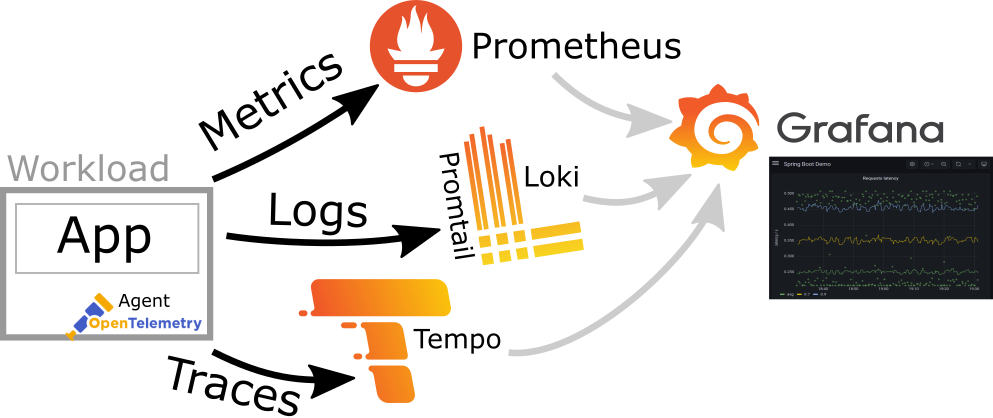
\includegraphics[scale=0.4]{./ressource/stackMonitoring}
\end{center}

\vspace{0.5cm}

\begin{encadre}{Métrique}
Mesure quantitative utilisée pour évaluer, surveiller et analyser les performances ou l'état d'un système, d'une application ou d'un processus. Elle peut inclure des données telles que la charge CPU, la mémoire utilisée, ou le temps de réponse d'un serveur.
\end{encadre}


Durant cette activité, nous allons mettre en place l'environnement de monitoring et étudier plus particulièrement \textbf{Prometheus} 

\subsection{Prometheus }
Prometheus est un système de surveillance open-source principalement utilisé pour collecter, stocker et analyser des métriques en temps réel.

\paragraph{Utilité principale}
\begin{itemize}
    \itemE Collecter des métriques à partir de divers systèmes ou applications (par exemple, l'utilisation de la CPU, la mémoire, le nombre de requêtes par seconde, etc.).
    \itemE Fournir une base de données de séries temporelles pour stocker ces métriques.
    \itemE Configurer des alertes basées sur des seuils prédéfinis.
\end{itemize}

\paragraph{Cas d'utilisation}
\begin{itemize}
    \itemE Surveiller les performances des applications et des infrastructures.
    \itemE Détecter les anomalies, les pics de charge ou les pannes.
\end{itemize}

\paragraph{Exemple}
Vous voulez savoir si votre serveur HTTP dépasse un certain taux de requêtes par seconde. Prometheus peut surveiller ce taux et déclencher une alerte si un seuil est atteint.

\vspace{0.5cm}
\begin{minipage}{0.75\linewidth}
\paragraph{Solutions alternatives : Zabbix}. C'est est une autre solution de surveillance open-source utilisée pour collecter des métriques, surveiller des applications et des infrastructures réseau en temps réel, ainsi que pour envoyer des alertes en cas de problèmes.
\end{minipage}
\begin{minipage}{0.25\linewidth}
\begin{center}

\includegraphics[scale=0.25]{./ressource/zabbix.png}
\end{center}
\end{minipage}

 Il permet de suivre les performances des systèmes, des serveurs et des équipements réseau grâce à des agents ou à des mécanismes de récupération comme SNMP. 
Comparé à Prometheus, Zabbix a une approche plus centralisé et traditionnelle ce qui le rend moins performant dans des environnements de micoservices et de conteneurs. Il sera étudié dans une prochaine activité.

\begin{encadre}{Microservices}
Architecture logicielle où une application est décomposée en plusieurs services indépendants responsable d'une fonctionnalité spécifique. Ces services communiquent généralement entre eux via des API et peuvent être développés, déployés, et mis à l'échelle de manière autonome.
\end{encadre}

\subsection{Loki}
Loki est un agrégateur de journaux (logs) développé par Grafana Labs. Contrairement à d'autres solutions comme ELK, Loki est conçu pour être léger et efficace.

\paragraph{Utilité principale}
\begin{itemize}
    \itemE Collecter et centraliser les journaux provenant de plusieurs sources (serveurs, conteneurs, applications).
    \itemE Permettre une recherche rapide et efficace dans ces journaux, en particulier lorsqu'ils sont reliés aux métriques.
\end{itemize}

\paragraph{Cas d'utilisation}
\begin{itemize}
    \itemE Identifier les erreurs ou exceptions dans les journaux d'une application.
    \itemE Corréler les événements dans les journaux avec des métriques.
\end{itemize}

\paragraph{Exemple}
Vous voulez comprendre pourquoi un service a échoué en analysant ses journaux. Loki vous permet de rechercher les logs spécifiques à cet incident.

\subsection{Tempo}
Tempo est un système de traçage distribué qui aide à suivre le cheminement d'une requête à travers plusieurs microservices au sein d'un système distribué.

\begin{encadre}{Système Distribué}
Ensemble de machines indépendantes (ordinateurs ou serveurs) qui coopèrent pour apparaître comme un système unique aux utilisateurs.  Ces machines partagent leurs ressources et communiquent via un réseau pour atteindre un objectif commun, tout en étant tolérantes aux pannes.
\end{encadre}



\paragraph{Utilité principale}
\begin{itemize}
    \itemE Fournir une vue d'ensemble des requêtes dans un système distribué.
    \itemE Identifier les goulets d'étranglement ou les latences dans les microservices.
\end{itemize}

\paragraph{Cas d'utilisation}
\begin{itemize}
    \itemE Diagnostiquer des problèmes de performance dans un environnement de microservices.
    \itemE Comprendre où et pourquoi une requête ralentit.
\end{itemize}

\paragraph{Exemple}
Une application utilisant plusieurs microservices présente une latence élevée. Tempo permet de visualiser le chemin exact d'une requête et de trouver quel service ou étape cause le problème.

\subsection{Grafana}
Grafana est un outil de visualisation puissant qui permet de créer des tableaux de bord interactifs pour afficher les données provenant de Prometheus, Loki, Tempo, et d'autres sources.

\paragraph{Utilité principale}
\begin{itemize}
    \itemE Visualiser les métriques, les journaux et les traces sous forme de graphiques, tableaux, et cartes.
    \itemE Configurer des alertes et surveiller les systèmes en temps réel.
\end{itemize}

\paragraph{Cas d'utilisation}
\begin{itemize}
    \itemE Centraliser toutes les données d'observabilité dans un seul tableau de bord.
    \itemE Fournir des graphiques intuitifs pour les équipes DevOps ou les managers.
\end{itemize}

\paragraph{Exemple}
Vous pouvez créer un tableau de bord montrant :
\begin{itemize}
    \itemE Les métriques des serveurs (CPU, RAM, etc. via Prometheus).
    \itemE Les journaux d'erreurs (via Loki).
    \itemE Les temps de réponse des requêtes (via Tempo).
\end{itemize}

\subsection{Résumé des rôles}


\footnotesize
\begin{center}

    \begin{tabular}{|l|l|l|}
        \hline
        \rowcolor{vert_capet}\textbf{Outil} & \textbf{Rôle Principal} & \textbf{Type de données gérées} \\
        \hline
        Prometheus & Surveillance des métriques (CPU, RAM, requêtes) & Séries temporelles \\
        Loki       & Analyse des journaux                             & Journaux (logs)    \\
        Tempo      & Suivi des requêtes dans les microservices       & Traces distribuées \\
        Grafana    & Visualisation des données et tableaux de bord  & Toutes les sources compatibles \\
        \hline
    \end{tabular}
\end{center}
\normalsize

\section{Dépôts utilisée}

Durant cette activités, vous allez utiliser trois dépôts : 

\begin{center}
 \rule{0.75\linewidth}{1pt}
 \end{center}
\begin{minipage}{0.6\linewidth}
\begin{itemize}
\itemE Dépôt contenant le \textbf{serveur IoT} en python que vous avez utilisé précédemment 
\end{itemize}
\href{https://github.com/PierreViland/serveurSimpleIot.git}{https://github.com/PierreViland/serveurSimpleIot.git}
\end{minipage}
\begin{minipage}{0.39\linewidth}

\begin{center}
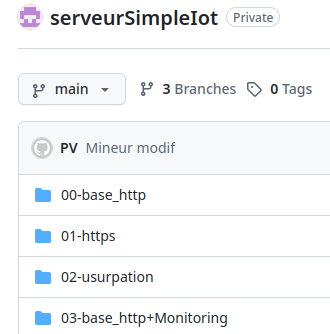
\includegraphics[scale=0.5]{./ressource/serveurIotGlobal}
\end{center}
\end{minipage}


\begin{center}
 \rule{0.75\linewidth}{1pt}
 \end{center}

\begin{minipage}{0.6\linewidth}
\begin{itemize}
\itemE Dépôt contentant les containers pour les \textbf{serveurs Nginx et apache} : 
\end{itemize}
\href{git@github.com:PierreViland/00-serveurLemp.git}{git@github.com:PierreViland/00-serveurLemp.git}
\end{minipage}
\begin{minipage}{0.39\linewidth}
\begin{center}
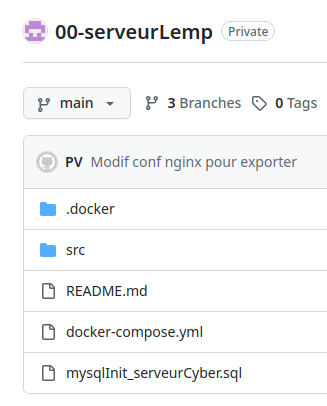
\includegraphics[scale=0.5]{./ressource/depotserveurGlobal}
\end{center}
\end{minipage}

\begin{center}
 \rule{0.75\linewidth}{1pt}
 \end{center}

\begin{minipage}{0.6\linewidth}
\begin{itemize}
\itemE Dépôt contenant les éléments pour mettre en place la \textbf{Monitoring stack} présent ici : 
\end{itemize}
\href{https://github.com/PierreViland/monitoringPV.git}{https://github.com/PierreViland/monitoringPV.git}
\end{minipage}
\begin{minipage}{0.39\linewidth}

\begin{center}
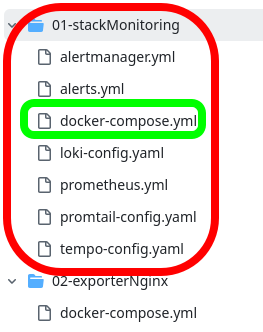
\includegraphics[scale=0.5]{./ressource/depo_global}
\end{center}
\end{minipage}

\section{Mise en place de la monitoring stack}
\begin{minipage}{0.6\linewidth}
Dans le dépot 

\href{https://github.com/PierreViland/monitoringPV.git}{https://github.com/PierreViland/monitoringPV.git} 

puis dans le répertoire \verb?01-stackMonitoring?, vous trouverez les le fichier \verb?docker-compose.yaml? et les différents fichiers de configuration de 
\begin{itemize}
\itemE Prometheus
\itemE Loki
\itemE Tempo
\itemE Grafana 
\end{itemize}
\end{minipage}
\begin{minipage}{0.39\linewidth}

\begin{center}
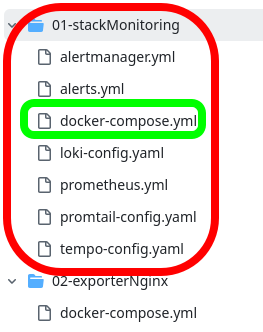
\includegraphics[scale=0.5]{./ressource/depo_global}
\end{center}
\end{minipage}



\vspace{0.5cm}

Nous allons nous intéresser dans un premier temps à \textbf{Prometheus et graffana}. Le système fonctionne de la sorte:
\begin{itemize}
\itemE \textbf{Collecte de métriques} : Prometheus interroge périodiquement (scrape) des endpoints HTTP exposant des métriques au format spécifique, souvent via des exportateurs (pour des services comme Nginx, MySQL, etc.
\itemE \textbf{Stockage des données} : Les métriques collectées sont stockées dans une base de données locale, optimisée pour les séries temporelles.
\itemE \textbf{Requêtes} : Prometheus permet aux utilisateurs d’interroger les données via son langage de requêtes PromQL (Prometheus Query Language) pour obtenir des informations et des statistiques détaillées.
\itemE \textbf{Alertes } : Il peut aussi être configuré pour envoyer des alertes en cas de seuils dépassés via des alertes Prometheus ou Alertmanager.
\itemE \textbf{Visualisation } Bien qu’il ne soit pas destiné à la visualisation, Prometheus est souvent couplé avec Grafana pour afficher graphiquement les métriques collectées
\end{itemize} 


\paragraph{Exemple de fonctionnement avec Nginx }

\begin{center}
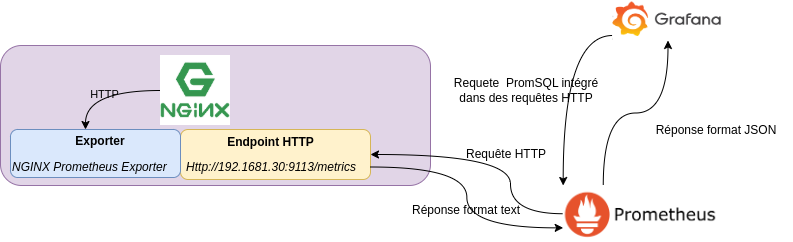
\includegraphics[scale=0.5]{./ressource/schemaPrometheus.drawio.png}
\end{center}
avec 

\begin{encadre}{Exporter}
Service qui expose des métriques d’un système (comme NGINX, MySQL, etc.) dans un format lisible par Prometheus.
\end{encadre}

\begin{encadre}{Endpoint}
URL (par exemple http://localhost:9113/metrics) à laquelle Prometheus accède pour scraper (collecter) les métriques fournies par un exporter.
\end{encadre}


\subsection{Exemple simple : serveur de température}

Dans une premier, vous allez exploiter \textbf{le serveur maison Iot}. L'objectif va être de récupérer des informations sur l'état du serveur tel que le nombre de connexion ou le temps moyen entre chaque connexion.  

En résumé, le système mise en place est le suivant

\begin{center}
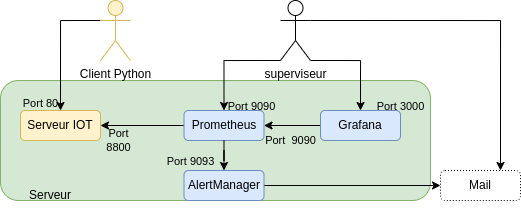
\includegraphics[scale=0.7]{./ressource/schemIotPrometeus.drawio.png}
\end{center}
avec
\begin{itemize}
\itemE \textbf{Client python}: script qui envoie une température (similaire à l'activité précédente)
\itemE \textbf{Serveur Python} : script python qui réceptionne les données (similaire à l'activité précédente)
\itemE \textbf{Prometheus} : container qui collecte les métriques exposées du serveur
\itemE \textbf{Grafana} : container permettant d'afficher sur une page web les métriques
\itemE \textbf{AlertManager} : container permettant de gérer les alertes (envoi de mail)
\itemE \textbf{Superviseur} : personne qui configure et visualise l'état du serveur
\end{itemize}


\vspace{0.5cm}
Si ce n'est pas déjà fait, vous pouvez le récupérer le client et le serveur python (comme dans l'activité précédente) dans le dépôt  
\begin{itemize}
\itemE \href{https://github.com/PierreViland/serveurSimpleIot.git}{https://github.com/PierreViland/serveurSimpleIot.git}
\end{itemize}


\vspace{0.5cm}
Vous pouvez soit utiliser la version HTTP (répertoire \verb?03-base_http+Monitoring? soit la version HTTPS (répertoire \verb?04-https+monitoring?)\footnote{Au 21/05/2025, il n'est pas encore créer $\Rightarrow$ A faire}. Dans tous les cas, les deux fichiers à exploiter sont : 

\begin{itemize}
\itemE le serveur : \verb?00-serveurPyhton.py?
\itemE le client : \verb?00-clientPythnTemperature.py?. Il n'a pas été modifié. Il sera juste utilisé. 
\end{itemize}

%\paragraph{Objectif} Nous voulons voir le nombre de connexion sur ce serveur (fichier \verb?00-serveurPyhton.py?)

\subsubsection{Exposition des métriques sur le serveur}

Dans le code python du serveur : 

\begin{itemize}
\itemE Un exportateur est crée via un serveur HTTP en début de fichier
\end{itemize}

\begin{lstlisting}[style=commande]
def start_prometheus_server():
    start_http_server(PROMETHEUS_PORT)
    print(f"Serveur Prometheus en ecoute sur le port {PROMETHEUS_PORT}...")
\end{lstlisting}


\begin{itemize}
\itemE Le serveur expose automatiquement les métriques disponibles au endpoint \verb?/metrics? via le port défini par \verb?PROMETHEUS_PORT? qui est : 
\begin{lstlisting}[style=commande]
PROMETHEUS_PORT = 8800  # Port pour exposer les metriques Prometheus
\end{lstlisting}



\itemE Les métriques exposées pour Prometheus sont  de plusieurs formes possibles :
	\begin{itemize}
	\item[+] \textbf{Counter} : Compte un événement qui ne peut qu'augmenter (ou être remis à zéro). Ex : Nombre total de requêtes, erreurs, etc.

	\item[+] \textbf{Gauge} : Mesure une valeur qui peut augmenter ou diminuer. Ex : Utilisation de mémoire, taille d'une file d'attente.				

	\item[+] \textbf{Histogram} : Regroupe des observations (comme des durées ou des tailles) dans des plages de valeurs (appelé buckets). Ex : Temps de réponse HTTP.

	\item[+] \textbf{Summary} : Similaire à un histogramme, mais calcule directement des quantiles (seuil spécifique entre 0 et 1) pour des observations. Ex : Temps moyen/percentile de traitement d'une requête.
\end{itemize} 
La documentation de la librairie Prometheus Pyhton est disponible ici : \\

 \href{https://prometheus.github.io/client_python }{https://prometheus.github.io/client\_python }

Dans notre cas, 3 métriques sont exposée (c.f \verb?00-serveurPyhton.py?)
\end{itemize}

\begin{lstlisting}[style=commande]
 19 # Creer un compteur pour les requetes POST
 20 post_requests_counter = Counter('http_post_nb_requete', 'Nombre total de requete POST')
 21 
 22 #Creation d'un historgramme pour le temps de reponse
 23 response_time_histogram = Histogram(
 24     'http_temps_reponse',
 25     'Histogramme des temps de reponse HTTP (s)',
 26     buckets=[0.001, 0.0015, 0.002, 0.003, 0.005, 0.0075]  # Definir les buckets pour l'histogramme
 27 )
 28 
 29 # Creer une metrique pour le temps ecoule entre les requetes
 30 time_between_requests_gauge = Gauge('http_time_between_requests_seconds', 'Temps entre chaque requete en secondes')

\end{lstlisting}



\begin{center}
 \rule{0.75\linewidth}{1pt}
 \end{center}
\begin{enumerate}
\item Lancer le serveur 
\begin{lstlisting}[style=commande]
sudo python3 00-serveurHttp.py
\end{lstlisting}

et le client 
\begin{lstlisting}[style=commande]
python3 01-clientEthernet.py
\end{lstlisting}


\item A l'aide d'un navigateur web observer les différentes métriques. 

\begin{lstlisting}[style=commande]
http://ip_addr:PROMETHEUS_PORT/metrics
\end{lstlisting}

\end{enumerate}
\begin{center}
 \rule{0.75\linewidth}{1pt}
 \end{center}

Ci-dessous un exemple de visualisation dans un navigateur :: 
\begin{center}
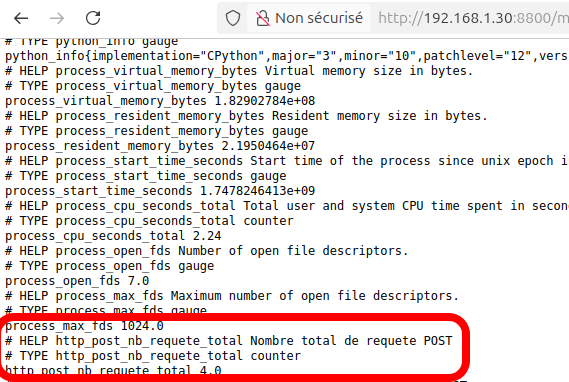
\includegraphics[scale=0.7]{./ressource/exPromServerIot}
\end{center}

Pour l'instant, les métriques sont accessibles mais non centralisées via Prometheus




\paragraph{Pour les élèves}
\begin{center}
 \rule{0.75\linewidth}{1pt}
 \end{center}
 \begin{itemize}
 \itemE Ils peuvent créer eux-même les métriques (compléter le code source)
 \end{itemize}
\begin{center}
 \rule{0.75\linewidth}{1pt}
 \end{center}



\ifPROF
\color{red}
\begin{lstlisting}[style=commande]  
 HELP http_post_nb_requete_total Nombre total de requete POST
# TYPE http_post_nb_requete_total counter
http_post_nb_requete_total 47.0
# HELP http_post_nb_requete_created Nombre total de requete POST
# TYPE http_post_nb_requete_created gauge
http_post_nb_requete_created 1.7358412745360215e+09
# HELP http_temps_reponse Histogramme des temps de reponse HTTP (s)
# TYPE http_temps_reponse histogram
http_temps_reponse_bucket{le="0.001"} 22.0
http_temps_reponse_bucket{le="0.0015"} 23.0
http_temps_reponse_bucket{le="0.002"} 44.0
http_temps_reponse_bucket{le="0.003"} 47.0
http_temps_reponse_bucket{le="0.005"} 47.0
http_temps_reponse_bucket{le="0.0075"} 47.0
http_temps_reponse_bucket{le="+Inf"} 47.0
http_temps_reponse_count 47.0
\end{lstlisting}

\normalcolor
\fi




\subsection{Lancement de la monitoring stack}

Nous allons maintenant lancer l'ensemble des service de monitoring. Pour rappel L'ensemble des fichiers relatifs à la "monitoring stack" est présent dans le répertoire \ \textbf{01-stackMonitoring} du dépôt  \href{https://github.com/PierreViland/monitoringPV.git}{https://github.com/PierreViland/monitoringPV.git}

Pour lancer correctement la monitoring stack, Il est nécessaire de regarder si le fichier de de configuration de Prometheus nommé \verb?prometheus.yml? est correct :

Il doit contenir au minimum les lignes suivantes (pour scraper les métriques de notre serveur maison) : 
\begin{lstlisting}[style=commande]
global:
  scrape_interval: 15s #Interval de recuperation des donnees
  
scrape_configs:
  - job_name: 'prometheus'
    static_configs:
      - targets: ['prometheus:9090']
      
  - job_name: 'serveurPython'
    static_configs:
      - targets: ['192.168.1.19:8800']  # Remplacez par l'adresse IP de votre serveur
\end{lstlisting}
avec
\begin{itemize}
\itemE Section \verb?global? : contient les paramètres globaux qui s'appliquent à toutes les configurations des \verb?scrape_configs?
\itemE Section \verb?scrape_configs? : liste les jobs (groupes de cibles) que Prometheus doit surveiller. Chaque job contient une liste de targets à interroger pour récupérer les métriques
	\begin{itemize}
	\item[$\Rightarrow$] \verb?job_name? nom du job (ex : serveurPython). Ce nom est utilisé pour identifier les métriques collectées de ce job.
	\item[$\Rightarrow$] \verb?static_configs?	: méthode pour définir statiquement les targets (adresses IP, noms d'hôtes, etc.).
	\item[$\Rightarrow$] \verb?targets?	: Liste des adresses où Prometheus doit collecter les métriques.
	\end{itemize}
\end{itemize}


\begin{center}
 \rule{0.75\linewidth}{1pt}
 \end{center}

\begin{enumerate}[resume]
\item Configurer le fichier \verb?prometheus.yml? pour que prometheus puisse récupérer vos données en modifiant les adresses IP et les port de vos cibles dans le fichier \verb?prometheus.yml?
\begin{lstlisting}[style=commande]
  - targets: ['@IP:Port'] 
\end{lstlisting} 


\item Lancer les conteneurs. Se mettre dans le répertoire \textbf{01-stackMonitoring}
\begin{lstlisting}[style=commande]
 sudo docker compose up -d
\end{lstlisting} 

\item Visualiser dans un navigateur web, l'ensemble des données de Prometheus. (Étudier le \verb?docker-compose.yaml? pour se connecter à Prometheus et surtout le port d'exposition de Prometheus).
\end{enumerate}


\begin{center}
 \rule{0.75\linewidth}{1pt}
 \end{center}

Si tous c'est bien déroulé, vous devez avoir une fenêtre similaire à celle ci-dessous.

\begin{center}
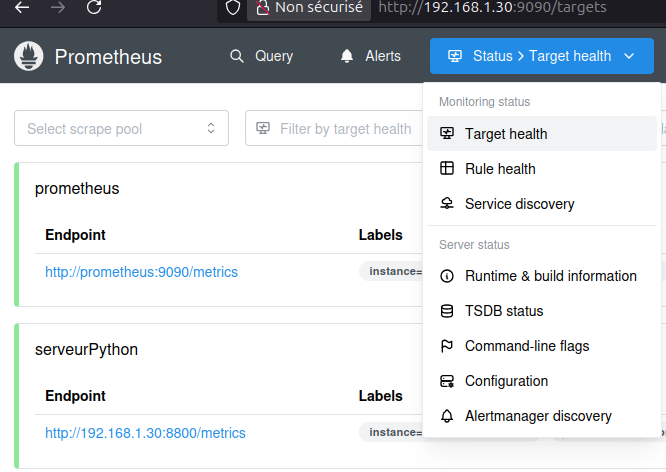
\includegraphics[scale=0.7]{./ressource/prometheus}
\end{center}


\ifPROF
\color{red}
\begin{lstlisting}[style=commande]  
Pour ce connecter : http://192.168.1.111:9090/

Il faut juste faire attention au port
\end{lstlisting}

\normalcolor
\fi


\subsection{Grafana}
Vous avez vu précédemment que \textbf{Prometheus} était adapté pour récupérer toutes sortes de métrique. \textbf{Grafana} va permettre d'afficher des  tableau de bord ("dashbord") pour afficher sour forme de graphique des rapports de monitoring. 



\begin{center}
 \rule{0.75\linewidth}{1pt}
 \end{center}

\begin{enumerate}[resume]
\item Se connecter à l'interface web de Grafana  (Étudier le \verb?docker-compose.yaml? pour se connecter à Prometheus). Les identifiants par défaut sont : 
	\begin{itemize}
	\item[$\Rightarrow$] Login : \verb?admin?
	\item[$\Rightarrow$] Mot de passe ! \verb?admin?
	\end{itemize}
\end{enumerate}


\begin{center}
 \rule{0.75\linewidth}{1pt}
 \end{center}
\ifPROF
\color{red}
\begin{lstlisting}[style=commande]  
Pour ce connecter : http://192.168.1.111:3000/
Il faut juste faire attention au port
\end{lstlisting}

\normalcolor
\fi

\begin{center}
 \rule{0.75\linewidth}{1pt}
 \end{center}

\begin{enumerate}[resume]
\item Ajouter et configurer une nouvelle source et effectuer la liaison avec Prometheus
\end{enumerate}


\begin{center}
 \rule{0.75\linewidth}{1pt}
 \end{center}
\begin{center}
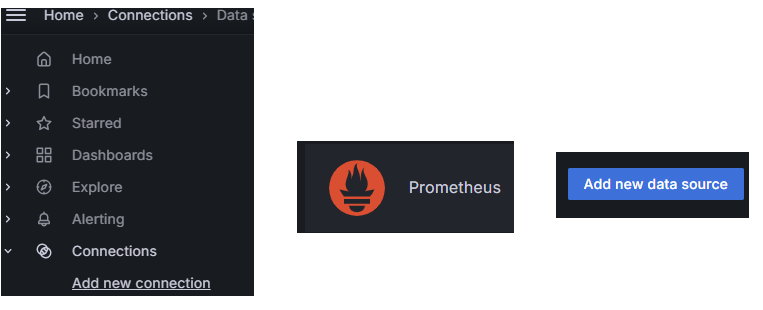
\includegraphics[scale=0.7]{./ressource/grafana_NewConnection.png}
\end{center}

%%%#https://blog.stephane-robert.info/docs/observer/metriques/prometheus/


\begin{center}
 \rule{0.75\linewidth}{1pt}
 \end{center}

\begin{enumerate}[resume]
\item Créer un nouveau dashboard et des nouveaux panels en fonction des métriques que vous voulez afficher.
\item Faire constater par votre professeur l'affichage de vos résultats. 
\end{enumerate}


\begin{center}
 \rule{0.75\linewidth}{1pt}
 \end{center}


\begin{center}
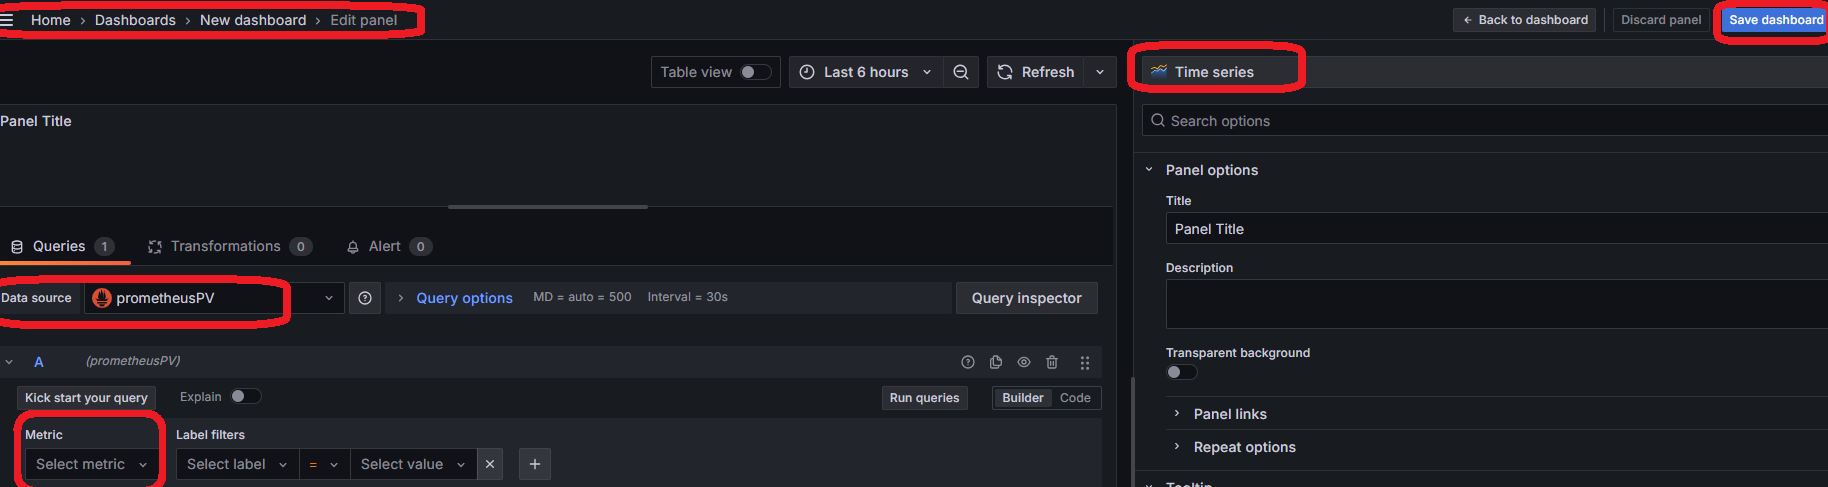
\includegraphics[scale=0.5]{./ressource/NewPanel.png}
\end{center}


\paragraph{Le résultat} du dashboard peut ressembler à cela

\begin{center}
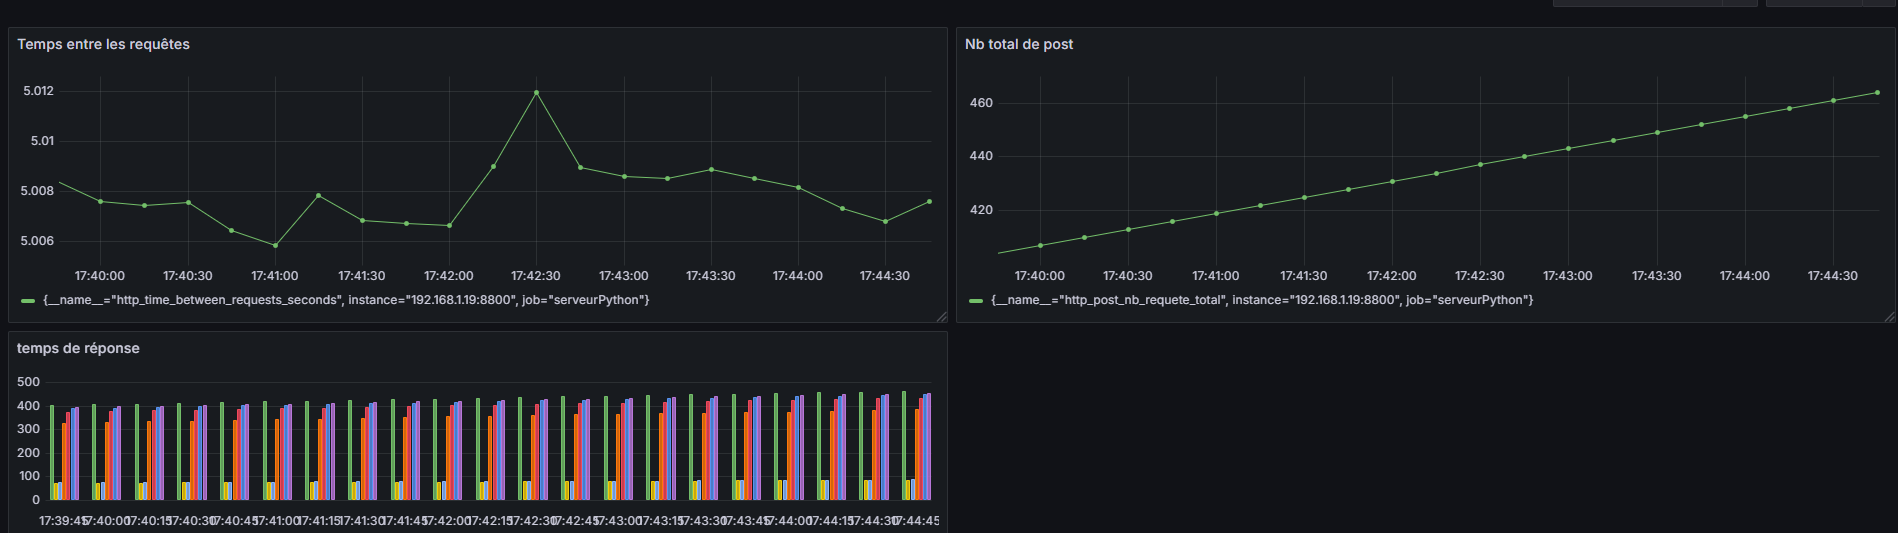
\includegraphics[scale=0.35]{./ressource/exPanel.png}
\end{center}


\section{Alerte}

L'alerte de Prometheus (Prometheus Alerting) est une fonctionnalité de Prometheus qui permet de surveiller des métriques et de générer des alertes lorsqu'une condition définie par l'utilisateur est remplie. Voici les points principaux à mettre en place (normalement en grande partie configurée dans le dépôt)  : 

\paragraph{Définir une Règle d'Alerte}
Les règles d'alerte sont définies dans un fichier de configuration nommé  \verb?alert.yml? qui est chargé par Prometheus. 

\begin{center}
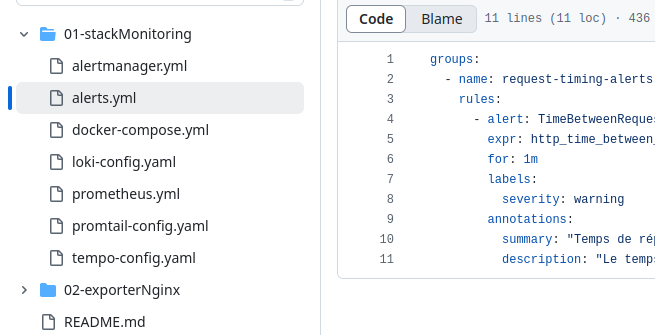
\includegraphics[scale=0.4]{./ressource/depot_alert_yml}
\end{center}

\begin{lstlisting}[style=commande]  
groups:
  - name: request-timing-alerts
    rules:
      - alert: TimeBetweenRequestsTooShort
        expr: http_time_between_requests_seconds < 4
        for: 1m
        labels:
          severity: warning
        annotations:
          summary: "Temps de reponse trop faible, attaque potentielle"
          description: "Le temps entre les requetes est trop faible (moins de 4 secondes), ce qui pourrait indiquer une attaque DDoS."
\end{lstlisting}


\begin{itemize}
\itemE \verb?alert? : Nom de l'alerte.
\itemE \verb?expr? : Expression PromQL pour définir la condition d'alerte.
\itemE \verb?for? : Durée pendant laquelle la condition doit être vraie pour déclencher une alerte.
\itemE \verb?labels? : Métadonnées pour catégoriser l'alerte (comme severity).
\itemE \verb?annotations? : Informations supplémentaires comme un résumé et une description.
\end{itemize}

\paragraph{Charger les Règles dans Prometheus} \ 

C'est le fichier \verb?prometheus.yml? qu'il faut configurer

\begin{center}
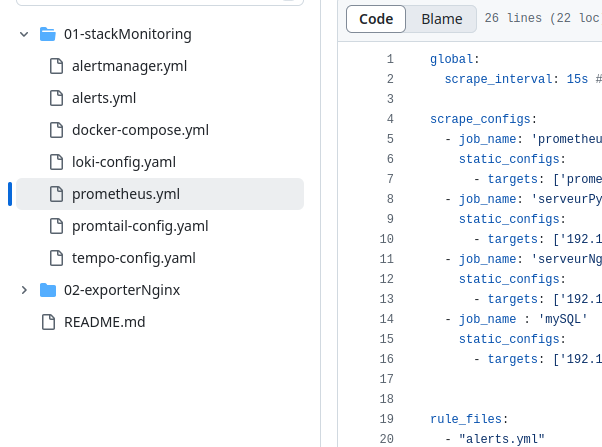
\includegraphics[scale=0.4]{./ressource/depot_prometheus_yml}
\end{center}

Les lignes suivantes doivent être présentes : 
\begin{lstlisting}[style=commande]  
rule_files:
  - "alerts.yml"
\end{lstlisting}

\paragraph{Configurer Alertmanager}
Vous devez configurer Alertmanager, qui recevra les alertes de Prometheus et les distribuera pour définir vos récepteurs (dans l'exemple e-mails) :


\begin{center}
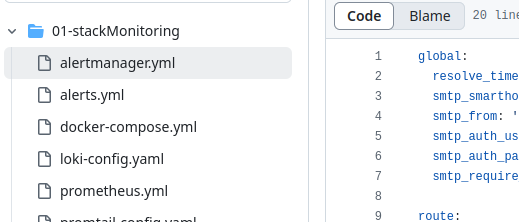
\includegraphics[scale=0.4]{./ressource/alertmanager}
\end{center}

\begin{lstlisting}[style=commande]  
global:
  resolve_timeout: 5m
  smtp_smarthost: 'smtp.gmail.com:587'
  smtp_from: 'xxxxxx@gmail.com'
  smtp_auth_username: 'xxxxx@gmail.com'
  smtp_auth_password: 'xxxx xxxx xxxx'  # Voir plus bas
  smtp_require_tls: true

route:
  receiver: "gmail-receiver"
  group_by: ['alertname']
  group_wait: 30s
  group_interval: 5m
  repeat_interval: 1h

receivers:
  - name: "gmail-receiver"
    email_configs:
      - to: "xxxxxx@ac-rennes.fr"
\end{lstlisting}


\paragraph{Configurer Prometheus pour utiliser Alertmanager}. Dans \verb?prometheus.yml?, ajouter (ou vérifier la présence de) une section pour pointer vers votre instance Alertmanager :

\begin{center}
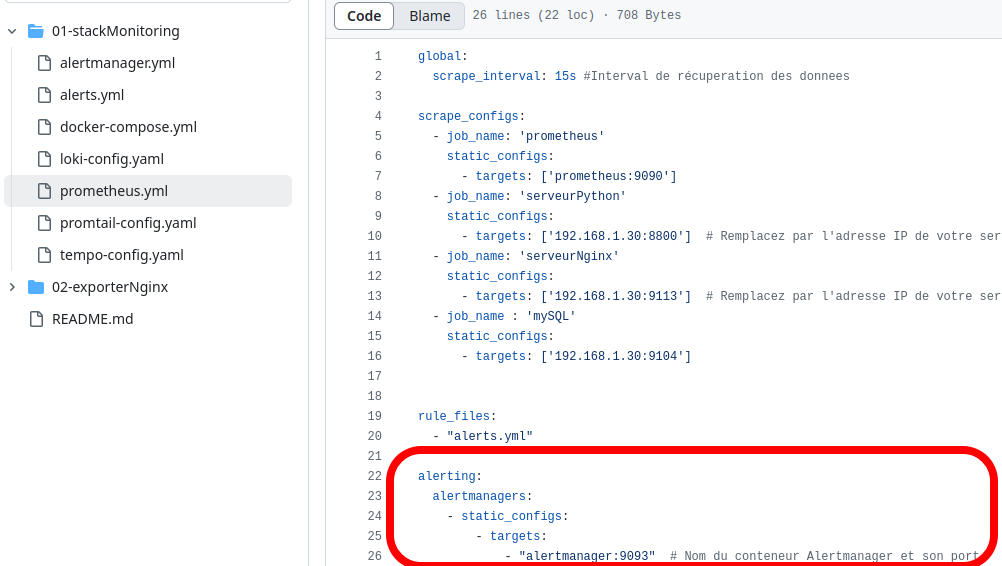
\includegraphics[scale=0.4]{./ressource/alertSouligne}
\end{center}

\begin{lstlisting}[style=commande]  
alerting:
  alertmanagers:
    - static_configs:
        - targets:
            - 'alertmanager:9093'
\end{lstlisting}
Ces lignes configure Prometheus pour qu’il envoie des alertes à un serveur "Alertmanager" qui écoute sur le port 9093 dès qu'une règle d'alerte est déclenchée.

\paragraph{le fichier docker-compose.yml} doit contenir les lignes permettant de lancer le container \verb?alertmanager?

\begin{center}
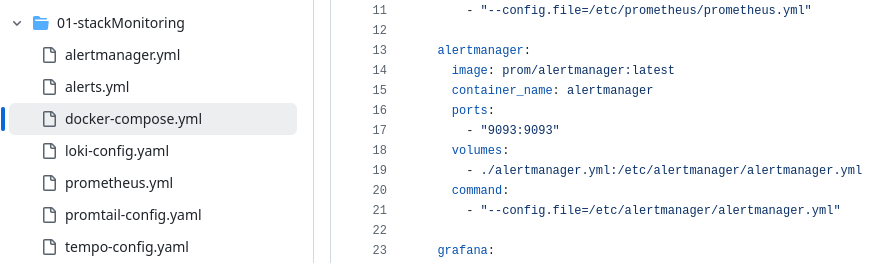
\includegraphics[scale=0.4]{./ressource/dockerAlert}
\end{center}

\begin{lstlisting}[style=commande] 
prometheus:
    image: prom/prometheus:latest
    container_name: prometheus
    ports:
      - "9090:9090"
    volumes:
      - ./prometheus.yml:/etc/prometheus/prometheus.yml
      - ./alerts.yml:/etc/prometheus/alerts.yml
    command:
      - "--config.file=/etc/prometheus/prometheus.yml"

  alertmanager:
    image: prom/alertmanager:latest
    container_name: alertmanager
    ports:
      - "9093:9093"
    volumes:
      - ./alertmanager.yml:/etc/alertmanager/alertmanager.yml
    command:
      - "--config.file=/etc/alertmanager/alertmanager.yml"
\end{lstlisting}      
     
     
\begin{center}
 \rule{0.75\linewidth}{1pt}
 \end{center}

\begin{enumerate}[resume]
\item Mettre en place l'alerte
\item La visualiser sur Prometheus
\item Configurer les mails pour recevoir l'alerte. (L'utilisation d'une adresse académique n'est pas possible. Par simplicité une adresse gmail "poubelle" est utilisé pour la démo \footnote{Il est nécessaire d'activer la double authentification sur le compte gmail puis obtenir créer un mot de passe d'application}
\end{enumerate}

\begin{center}
 \rule{0.75\linewidth}{1pt}
 \end{center}
 


Le résultats d'exécution : est : 

\begin{center}
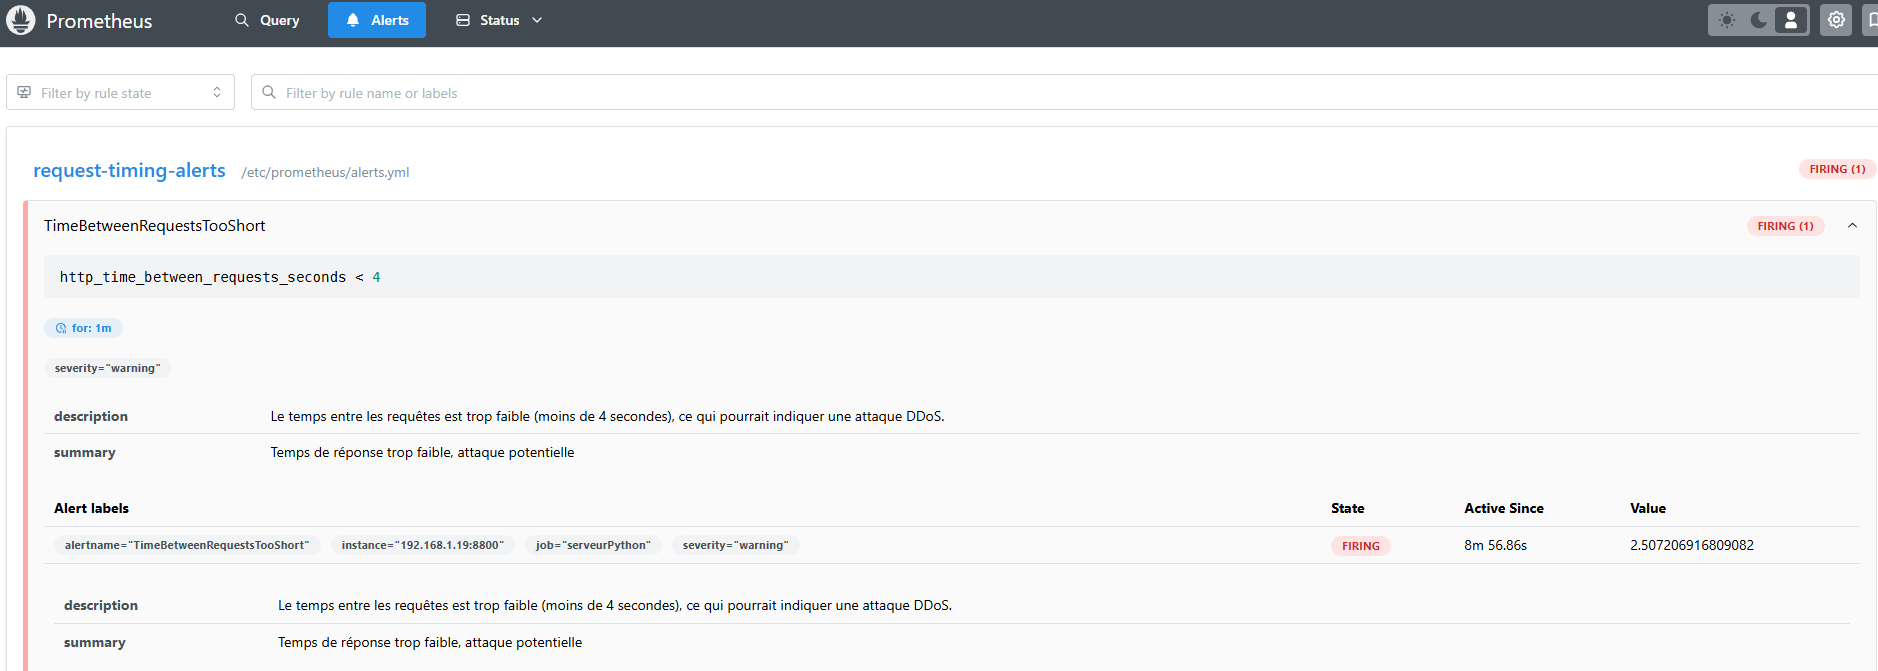
\includegraphics[scale=0.4]{./ressource/AlertPrometheuse}
\end{center}


\begin{center}
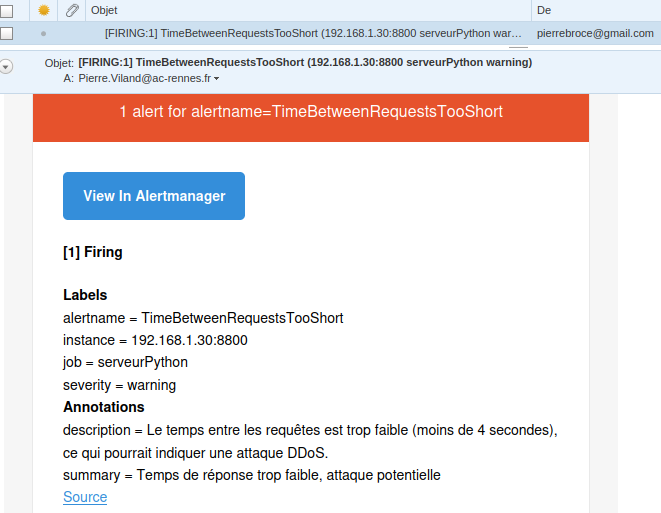
\includegraphics[scale=0.6]{./ressource/resMail}
\end{center} 
 

 
 
\section{Métrique LEMP}
Vous avez scruté les métriques d'un serveur "maison".  Il est possible de scruter des services professionnels comme notre serveur LEMP. 


\begin{center}
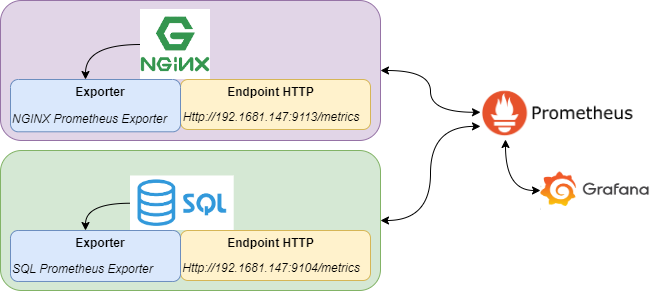
\includegraphics[scale=0.7]{./ressource/schemaPrometheus-LEMP_Prometheuse.drawio.png}
\end{center}

Les différents fichier de configuration sont présent en ressource dans le répertoire : \verb?02-LEMP_monitoring+serveurPyhton?


\paragraph{Lancement des "exporters"}
Il faut commencer par créer deux containers correspondant aux deux exporter
\begin{itemize}
\itemE \verb?NGINX Prometheus?
\itemE \verb?SQL Prometheus?
\end{itemize}


Un fichier de \verb?docker-compose.yml? est présent dans le répertoire \verb?02-exporter?
\begin{center}
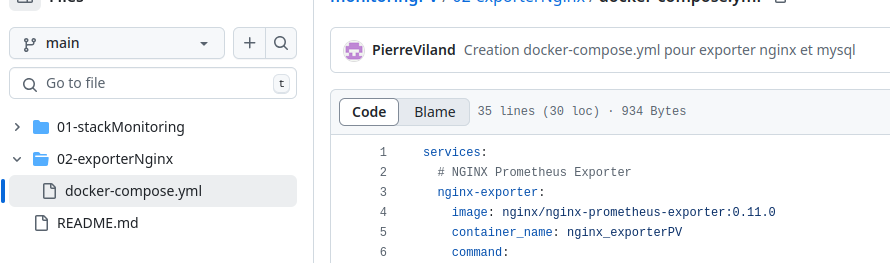
\includegraphics[scale=0.4]{./ressource/visuDockerExporter}
\end{center}
Ce fichier permet de lancer les exporters du Nginx et MySQL. Il faudra le lancer via la commande
\begin{lstlisting}[style=commande]
sudo doker compose  up -d
\end{lstlisting}



\paragraph{Création des jobs} \ 

Il faut ensuite, ajouter deux jobs dans \verb?prometheus.yml? pour que le service  Prometheus surveille \verb?Nginx? et \verb?MySql?
\begin{lstlisting}[style=commande] 
  - job_name: 'nginx'
    static_configs:
      - targets: ['@IP_LEMP:9113']

  - job_name: 'mysql'
    static_configs:
      - targets: ['@IP_LEMP:9104']    
}
\end{lstlisting} 

\begin{center}
 \rule{0.75\linewidth}{1pt}
 \end{center}



\paragraph{Configuration de Nginx}\ 

Il faudra ensuite vérifier que le fichier de configuration de NGINX

(\verb?00-serveurLemp\.docker\nginx\conf.d\default.d? contienne les lignes suivantes
\begin{lstlisting}[style=commande] 
server {
     listen 9114;
     server_name localhost;
 
     location /nginx_status {
         stub_status;
         allow all;   #Attention pas secu
     }
}
\end{lstlisting} 

Ces lignes ouvrent le port 9114 pour récupérer les métriques des nginxs. \textbf{Attention, ce n'est plus le dépôt relatif au serveur LEMP}

\begin{center}
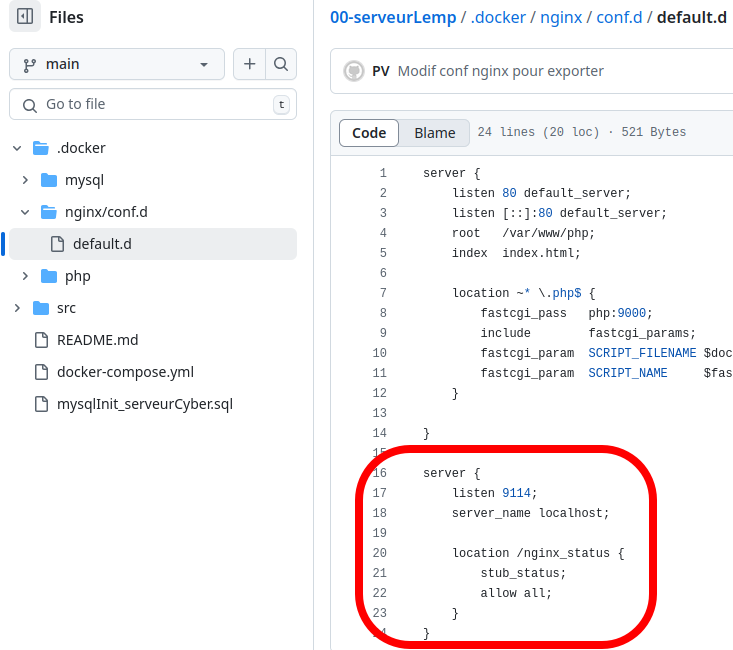
\includegraphics[scale=0.4]{./ressource/verifNginx}
\end{center}



\begin{center}
 \rule{0.75\linewidth}{1pt}
 \end{center}
\begin{enumerate}[resume]
\item Mettre la surveillance de Nginx et de MySql
\item Appeler le professeurs pour visualiser vos résutlats
\item En fonction des métriques récupérées, afficher des éléments importants dans Grafana
\end{enumerate}

\section{Métrique sécurisé}

\subsection{Présentation}

Jusqu'à présent, nous utilisons \textbf{un exporter exposant un endpoint}, que Prometheus vient interroger (scraper) pour collecter les métriques. Toutes les communications s’effectuent en HTTP.

Prometheus peut interroger un ensemble de services, même s'ils ne se trouvent pas sur le même système d'exploitation. Par exemple, vous pouvez scraper le serveur d'un autre hôte, à condition qu'il vous fournisse l'adresse IP et le port de son endpoint.

Cependant, cela pose un problème de sécurité : les communications ne sont pas chiffrées, et le endpoint n'est pas authentifié. Pour y remédier, une démarche courante est de placer un \textbf{reverse proxy} capable de gérer le chiffrement (HTTPS) et l'authentification. 


\begin{encadre}{reverse proxy}
Serveur intermédiaire qui reçoit les requêtes des clients et les redirige vers les serveurs en arrière-plan, tout en pouvant gérer des fonctionnalités comme le chiffrement HTTPS, l'authentification ou la répartition de charge.
\end{encadre}

Le schéma ci-dessous résume cette solution. 

\begin{center}
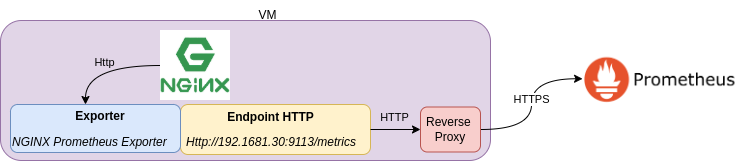
\includegraphics[scale=0.6]{./ressource/schemaHTTPSPrometheus.drawio.png}
\end{center}

\subsection{Mise en place}

Dans cette partie nous allons mettre en place une communication sécurisée et déacitver la non sécurisé  entre 
\begin{itemize}
\itemE \verb?Prometheus? $\Leftrightarrow$ \verb?Exporter Nginx?
\itemE \verb?Un client Web? $\Leftrightarrow$ \verb?Prometheus?
\end{itemize}

Pour être pleinement opérationnel, nous pourrions aussi faire de même pour le serveur sql et le serveur IOT. 


\subsubsection{Stopper les machines}

Plusieurs modifications doivent être réalisées pour pouvoir utiliser le reverse proxy. Il faut donc stopper les containers relatifs à 
\begin{itemize}
\itemE Prometheus  présent dans le répertoire 

\verb?https://github.com/PierreViland/monitoringPV/tree/main/01-stackMonitoring?
\itemE L'exporters de Nginx présent dans le répertoire : 

 \verb?https://github.com/PierreViland/monitoringPV/tree/main02-exporterNginx?
\end{itemize}

\begin{center}
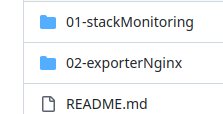
\includegraphics[scale=0.5]{./ressource/repMonitoring}
\end{center}

Sur votre VM, dans chacun des répertoires stopper les containers à l'aide de la commande : 

\begin{lstlisting}[style=commande] 
$ sudo docker compose down
\end{lstlisting} 

Normalement, seul les containers du service web sont lancés. Vous pouvez vérifier à l'aide  de la commande suivante.
\begin{lstlisting}[style=commande] 
$ sudo docker compose ps
\end{lstlisting} 


\subsubsection{Changement de branches}

Etant un chic type, je vous fourni la configuration de notre système avec un reverse proxy. 
Pour cela, il suffit de changer de branche

\begin{lstlisting}[style=commande] 
~/05-monitoring/monitoringPV$ git branch 
* main
  secureMonitoring
~/05-monitoring/monitoringPV$ git switch secureMonitoring 
Switched to branch 'secureMonitoring'
Your branch is up to date with 'origin/secureMonitoring'.
\end{lstlisting} 

Le répertoire \textbf{03-reverse/} est apparu. Il contient le fichier \verb?docker-compose.yml ? relatif au reverse Proxy. 

\subsubsection{Configuration}

\paragraph{01-StackMonitoring}

Ce paragraphe montre les modification de containers prometheus \textit{"pour passer en HTTPS"}
\begin{center}
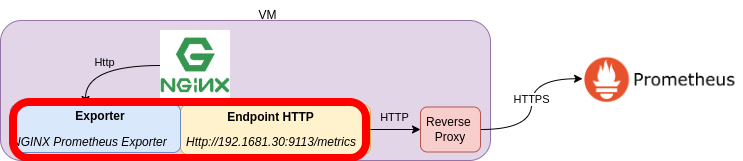
\includegraphics[scale=0.5]{./ressource/etapeStackMonitoring.png}
\end{center}

Il est nécessaire de préciser au container prometheus que l'url extérieur a changer et qu'il y aura un préfixe pour la redirection de port. les lignes suivantes doivent être modifiées (surtout) l'IP : 

\begin{lstlisting}[style = commande]
 services:                                                                                                                                                                                 
   prometheus:
     image: prom/prometheus:latest
     container_name: prometheus
     #ports:                     #A enelver pour que l'on ne voit plus le port HTTP (derriere le reverse proxy)
     #  - "9090:9090"
     volumes:
       - ./prometheus.yml:/etc/prometheus/prometheus.yml
       - ./alerts.yml:/etc/prometheus/alerts.yml
     command:
       - "--config.file=/etc/prometheus/prometheus.yml" #Indique l'emplacement du fichier de conf
       - '--web.route-prefix=/'                         #Indique le prefix de l'url de prometheus. A faire si reverse Proxy
       - '--web.external-url=https://192.168.1.30:4433' #Url de point d'entree de prometheus. A faire si reverse Proxy 

\end{lstlisting}

Le reste de la \verb?stack monitoring? n'est pas à modifier sauf si vous voulez la sécurisée.


\paragraph{02-exporterNginx}
Ce paragraphe montre les modification de l'exporter nginx pour \textit{"pour passer en HTTPS"}
\begin{center}
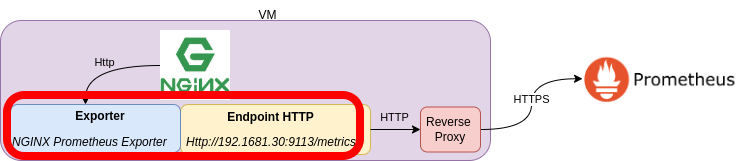
\includegraphics[scale=0.5]{./ressource/etapeExporter.png}
\end{center}

Dans le \textbf{docker-compose.yml},  il est nécessaire de commenter les lignes qui permette l'exposition du port du container vers l'extérieur.

\begin{lstlisting}[style = commande]
services:                                                                                                                                                                                     
  # NGINX Prometheus Exporter
  nginx-exporter:
    image: nginx/nginx-prometheus-exporter:0.11.0
    container_name: nginx_exporterPV
    command:
      - --nginx.scrape-uri=http://nginxPV:9114/nginx_status
    #ports:   # A supprimer lorsque reverse proxy. On ne redirige pas le port sur l'hote
    #  - "9113:9113"
    networks:
      - mynet
\end{lstlisting}


Il faut bien veiller à avoir en fin de fichier le partage du réseau avec les autres containers 

\begin{lstlisting}[style = commande]
networks:
  mynet:
    external: true  # Indique que le reseau existe deja
    name: 00-serveurlemp_mynet # Nom explicite du reseau existant
\end{lstlisting}

\paragraph{03-reverse}
Ce paragraphe montre la création d'un reverse proxy pour faire l'interface entre les éléments du réseau containerisé \verb? 00-serveurlemp_mynet? et "le monde extétrieur.
\begin{center}
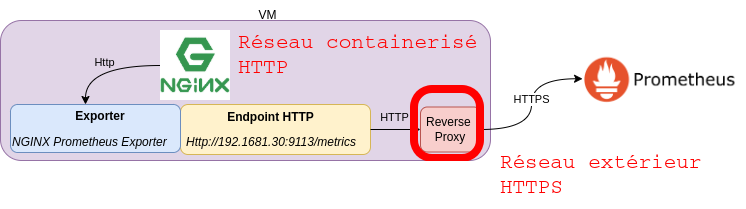
\includegraphics[scale=0.5]{./ressource/etapeReverse.png}
\end{center}

Le reverse proxy est basé sur un serveur Nginx (une autre instance de celui dédié aux pages web)

Dans le répertoire \textbf{03-reverse},trois fichiers sont présents et doivent être configurés en fonction des besoins. Il permettent de faire la redirection automatique entre les requête HTTPS avec des 

\begin{itemize}
\itemE \verb?docker-compose.yml?
\end{itemize}
Ce fichier "lance" un container Nginx en exposant les ports 8008 (http) et 4433 (https) sur le réseau extérieur ce seront ces ports qui seront utilisés pour accéder de manière sécurisé au métrique du serveur web.


\begin{lstlisting}[style = commande]
 5     ports:
 6       - "8008:8008"
 7       - "4433:4433"
\end{lstlisting}

De plus, ce container partage avec l'hote de répertoire contant respectivement, 
\begin{itemize}
\item[ ] 
\begin{itemize}
\item[+] le fichier de configuration du reverse proxy 
\item[+] la clefs et le certificat du reverse proxy
\end{itemize}
\end{itemize}

\begin{lstlisting}[style = commande]
  8     volumes:
  9       - ./nginx.conf/nginx.conf:/etc/nginx/nginx.conf:ro
 10       - ./cert/:/etc/nginx/certs/:ro
\end{lstlisting}


Il faut bien veiller à avoir en fin de fichier le partage du réseau avec les autres containers 

\begin{lstlisting}[style = commande]
networks:
  mynet:
    external: true  # Indique que le reseau existe deja
    name: 00-serveurlemp_mynet # Nom explicite du reseau existant
\end{lstlisting}



\begin{center}
 \rule{0.75\linewidth}{1pt}
 \end{center}


\begin{itemize}
\itemE \verb?./cert/geneCertClef.sh?
\end{itemize}
Ce fichier génère un certificats et une clef pour le reverse proxy.

Dans le fichier présent sur le dépôt, la CA est celle utilisé pour le HTTPS du serveur WEB de la précédente activité.	(ligne 4 -5)

\begin{lstlisting}[style = commande]
  1 #!/bin/bash                                                                                                                                                                               
  2 
  3 # Definition des fichiers
  4 CA_KEY="../../../../../00-serveurLemp/openSSL/ca.key"   #Clef privee du CA
  5 CA_CERT="../../../../../00-serveurLemp/openSSL/ca.crt"  #Certificat du CA

\end{lstlisting}

Si vous souhaitez générer une nouvelle CA les lignes 22 et 25 doivent être décommentée.

\begin{lstlisting}[style = commande]
#Ligne commenter car reutilisation d'une CA existante
 20 # Creation de la CA SI VOUS VOULEZ UN NOUVEAU CA => Decommente
 21 #echo "Creation de la cle privee de la CA..."
 22 #openssl genrsa -out $CA_KEY 2048
 23 
 24 #echo "Creation du certificat auto-signe de la CA..."
 25 #openssl req -x509 -new -key $CA_KEY -sha256 -days 3650 -out $CA_CERT -subj "/CN=$CA_CN"
\end{lstlisting}

Le noms du certificat et de la clef générés sont définis respectivement ligne 9 et 7

\begin{lstlisting}[style=commande]
  7 SERVER_KEY="reverseProxy.key"  #Clef privee du serveur
  8 SERVER_CSR="reverseProxy.csr"  #Certificat du serveur en attente de signature Certificate Signing Request
  9 SERVER_CERT="reverseProxy.crt" #Certificat du serveur
 10 SERVER_EXT="reverseProxy.ext"  #Contient des options pour la generation du certificat serveur (pas utilise apres)
\end{lstlisting}



\begin{center}
 \rule{0.75\linewidth}{1pt}
 \end{center}

\begin{itemize}
\itemE \verb?./nginx.conf/nginx.conf/?
\end{itemize}

Ce fichier permet de configurer \textbf{nginx} pour qu'il fonctionne en reverse proxy.

\begin{itemize}
\item[ ] 
\begin{itemize}
\item[+] On retrouve le certificat et la clef pour les connexions HTTPS
\end{itemize}
\end{itemize}
\begin{lstlisting}[style=commande]
 12         ssl_certificate /etc/nginx/certs/reverseProxy.crt;
 13         ssl_certificate_key /etc/nginx/certs/reverseProxy.key;
\end{lstlisting}


\begin{itemize}
\item[ ] 
\begin{itemize}
\item[+] Pour chaque service HTTP que l'on souhaite protéger, on va retrouver une structure comme ci-dessous : 
\end{itemize}
\end{itemize}
\begin{lstlisting}[style=commande]
 22         location /nginx-metrics/ {
 23             proxy_pass http://nginx_exporterPV:9113/;
 24             proxy_set_header Host $host;
 25             proxy_set_header X-Real-IP $remote_addr;
 26             proxy_redirect off;
 27         }
\end{lstlisting}
Ces lignes définissent une route \verb?/nginx-metrics/? à mettre dans l'URL qui redirige les requêtes vers le container \verb?nginx_exporterPV? écoutant sur le port 9113 (exporter de mon service web). Il faut bien veiller à avoir tous les containers sur le même réseau containerisé.

\subsubsection{Lancement}

Il est maintenant nécessaire de lancer l'intégralité des containers. Pour cela, il faut se placer dans chacun des répertoires 
\begin{itemize}
\itemE \verb?01-stackMonitoring?
\itemE \verb?02-exporterNginx?
\itemE \verb?03-reverse?
\end{itemize}
et exécuter la commande qui permet de construire et lancer les containers 

\begin{lstlisting}[style=commande]
docker compose up -d
\end{lstlisting}

Si tous fonctionne vous devez avoir accès a la page suivante 

\begin{center}
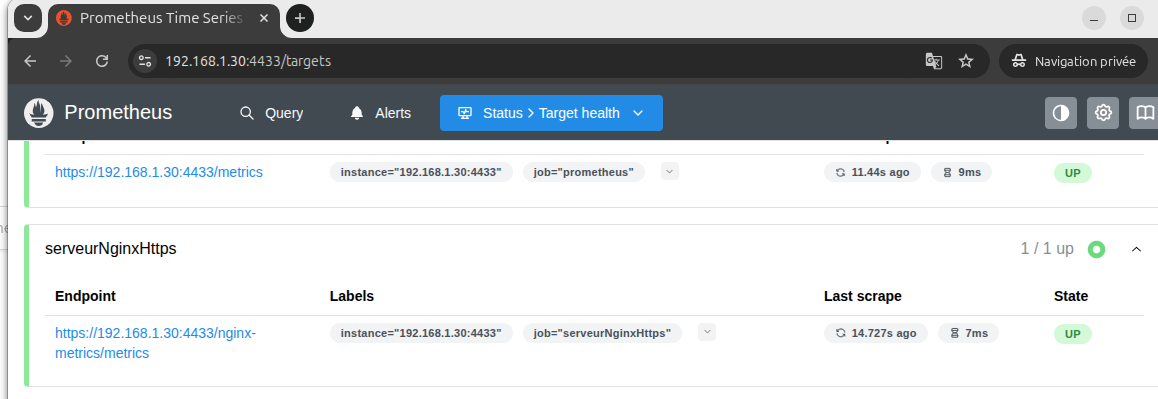
\includegraphics[scale=0.6]{./ressource/finalPromHTTPS}
\end{center}



\section{Suite et conclusion}

Nous avons vu : 
\begin{itemize}
\itemE Le monitoring de service via a prometheus
\itemE La sécurisation de ces échanges via un reverse proxy 
\end{itemize}

Pour aller plus loin, il serait possible de : 
\begin{itemize}
\itemE Finir de sécurisé l'intégralité des services
\itemE Monitorer d'autres services (exemple apache)
\end{itemize}


\end{document}
